\documentclass[final,hyperref={pdfpagelabels=false}]{beamer}
\usepackage{grffile}
\mode<presentation>{\usetheme{I6pd2}}
\usepackage[english]{babel}
%\usepackage{natbib}
\usepackage[latin1]{inputenc}
\usepackage{amsmath,amsthm, amssymb, latexsym}
\boldmath
\usepackage[orientation=landscape,size=a0,scale=1.2,debug]{beamerposter}
\usepackage{array,booktabs,tabularx}
\newcolumntype{Z}{>{\centering\arraybackslash}X}
\newcommand{\pphantom}{\textcolor{ta3aluminium}}

\listfiles
 
\title{\LARGE Big Data Analytics Pipeline for the Analysis of TESS Full Frame Images}
\author{Matthew Wampler-Doty \& Dr. John Doty}
\institute[Noqsi Aerospace]{Noqsi Aerospace, Ltd. \& MIT}
\date[]{}
\newlength{\columnheight}
\setlength{\columnheight}{105cm}

\begin{document}
\begin{frame}
  \begin{columns}
    \begin{column}{.49\textwidth}
      \begin{beamercolorbox}[center,wd=\textwidth]{postercolumn}
        \begin{minipage}[T]{.95\textwidth}  % tweaks the width, makes a new \textwidth
          \parbox[t][\columnheight]{\textwidth}{
            \begin{block}{Introduction}
            The goals of this research are two fold:
              \begin{itemize}
              \item Create a \emph{fast, high fidelity} simulation of the TESS Full Frame Images (FFI)
              \item Develop data processing system that takes the TESS FFIs and looks for items such as:
              \begin{itemize}
              	\item Tidal disruption events
	        \item Gamma-ray burst afterglow
		\item Low surface brightness structures
		\item Unusual variable objects
		\item Exoplanets around non-targeted stars
              \end{itemize}
              \end{itemize}              
            \end{block}

            \vspace{2cm}
            \begin{block}{Conventional Data Processing Pipeline}
            \begin{itemize}
              	\item Conventional processing for astronomical data attempts to scrub out artifacts and then extract results from clean images.
		\item Computational requirements are relatively low, but the scrubbing process may remove real effects and makes error estimates less accurate.
		\item In the past, the approach was necessary due to the high expense of computation.
	    \end{itemize}
              
\includegraphics[width=0.95\linewidth]{figures/Conventional_Pipeline.pdf}
            \end{block}

            \vspace{2cm}
            \begin{block}{Our Intended Simulation-Driven Processing Loop}
            Running a model through a simulation to compare with the rawest data available is statistically more robust, in theory. In order get good agreement every significant effect must be included in the model, whether you consider it an intended data product or an `artifact'. This makes it harder to ignore unexpected events and phenomena. Running multiple simulations is computationally expensive, but with the cost of Gflop/s cores at  $\approx$\$0.20/core and falling rapidly, this is manageable.
              \begin{center}
              
\includegraphics[width=0.75\linewidth]{figures/Our_Pipeline.pdf}
              \end{center}
            \end{block}
          }
        \end{minipage}
      \end{beamercolorbox}
    \end{column}
    % ---------------------------------------------------------%
    % end the column

    % ---------------------------------------------------------%
    % Set up a column 
    \begin{column}{.49\textwidth}
      \begin{beamercolorbox}[center,wd=\textwidth]{postercolumn}
        \begin{minipage}[T]{.95\textwidth}
          \parbox[t][\columnheight]{\textwidth}{
            \begin{block}{Simulated TESS Full Frame Image}
            Image generated by Zach Berta-Thompson using his existing simulator
              \begin{columns}
                \begin{column}{.60\textwidth}
                \begin{itemize}
                    \item In our new simulator, the \emph{Sky Model} will include catalog stars, galaxies, solar system bodies, diffuse galactic light, zodiacal light, ...
                    \vfill
                    \item We will simulate optics, CCD detector physics, and electronics.
                    \begin{itemize}
                    	\item Every photon from every star is independent, so we can rapidly generate an image using parallelization technologies like \texttt{CUDA} 
			\item We can further accelerate the process by choosing a representative sample of photon paths and weighting. This can also yield a more accurate estimate of the expectation value than a straight Monte Carlo simulation.
                    \end{itemize}
                    \vfill
                    \item We will also simulate the TESS on-board data processing, including the cosmic ray scrubbing to be applied to the FFIs.
                    \vfill
                \end{itemize}
                \end{column}
                \begin{column}{.38\textwidth}
                  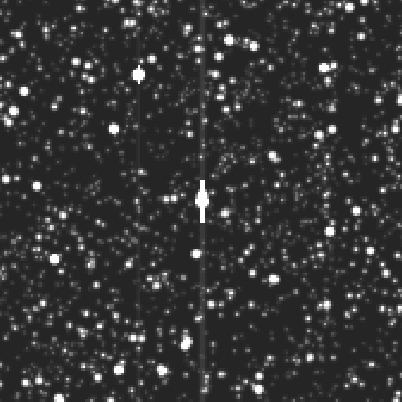
\includegraphics[width=0.80\linewidth]{figures/ffi_simulation.jpg}
		\end{column}
	       \end{columns}
            \end{block}
            \vspace{1cm}
            \begin{block}{Evaluation}
            	\begin{itemize}
			\item Series of images give rise to time series which can be mined looking for various objects and events
			\item To evaluate the performance of a particular data mining algorithm, downlink data is simulated 
			\item Comparison of algorithms uses various statistical performance measurements, such as $F_1$ scores, \emph{Markedness}, \emph{Informedness}, Area under ROC Curve and others
				\begin{columns}
                			\begin{column}{.30\textwidth}
			        $$ F_1 = \frac{A}{A + \frac{B + C}{2}} $$
			       
			       $$ Markedness = \frac{A}{A + B} + \frac{C}{C+D}$$
			       
			       $$ Informedness = \frac{A}{A+C} + \frac{B}{B+D}$$
			       \end{column}
                		       \begin{column}{.38\textwidth}
		                         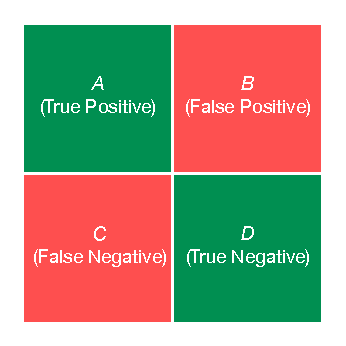
\includegraphics[width=0.65\linewidth]{figures/truth_table}
	       		       \end{column}
			       \end{columns}
			       \begin{columns}
			       \begin{column}{.60\textwidth}
			       Hurst exponent explanation goes here \cite{hurst_long-term_1951} 
			       \end{column}
			       \begin{column}{.38\textwidth}
			       	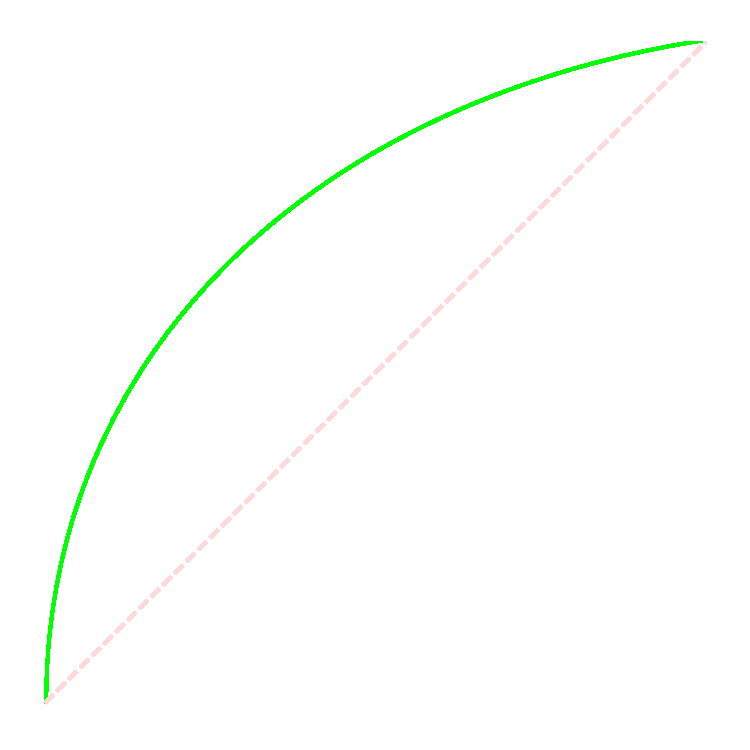
\includegraphics[width=0.65\linewidth]{figures/ROC}
			       \end{column}
			       \end{columns}
                \end{itemize}
            \end{block}
            \begin{block}{Bibliography}
	   \bibliographystyle{plain}
            \bibliography{./bibliography.bib}
            \end{block}
          }

        \end{minipage}
      \end{beamercolorbox}
    \end{column}
    % ---------------------------------------------------------%
    % end the column
  \end{columns}
  \vskip1ex
  \tiny\hfill{Created with \LaTeX \texttt{beamerposter}  \url{http://www-i6.informatik.rwth-aachen.de/~dreuw/latexbeamerposter.php} \hskip1em}
\end{frame}
Project Plan

Primarily a software project.

Small team, open source, highest productivity 21st century methodology.

Outside contributions are welcome.

Database of results freely accessible.

Give URL of GitHub project here.

The authors acknowledge productive discussions with Garrett Jernigan, Roland Vanderspek, and George Ricker.
%
\end{document}

%%%%%%%%%%%%%%%%%%%%%%%%%%%%%%%%%%%%%%%%%%%%%%%%%%%%%%%%%%%%%%%%%%%%%%%%%%%%%%%%%%%%%%%%%%%%%%%%%%%
%%% Local Variables: 
%%% mode: latex
%%% TeX-PDF-mode: t
%%% End:
